\documentclass[11pt]{article}

\usepackage{graphicx} %Required for diagrams
\usepackage[export]{adjustbox} %Required to Adjust Image alignment
\usepackage{float}
\usepackage[bookmarks=true]{hyperref}
\usepackage{bookmark}%Required to do pdf bookmarking
\usepackage{hyperref}%Required for referencing website pages

\begin{document}


\begin{titlepage}
\begin{center}

\includegraphics[width=350px]{University_of_Pretoria_Logo.png}\newline
% Title
\textsc{\LARGE COS301 Mini Project Functional Requirements Specification}\newline


%\begin{minipage}{0.4\textwidth}
\textbf{Group 4B} \\
\begin{flushright} \large
Kyhle Ohlinger \emph{u11131952} \newline
Andrew Parkes \emph{u12189139} \newline
Sifiso Shabangu \emph{u12081622} \newline
New Member \emph{uxxxxxxxx} \newline
New Member \emph{uxxxxxxxx} \newline
New Member \emph{uxxxxxxxx} \newline
New Member \emph{uxxxxxxxx} \newline \newline \newline
\end{flushright}
%\end{minipage}
Here's a link to \href{https://github.com/KyhleOhlinger/COS301-Group-4_B.git}{Github}.


\vfill

{\large Version 1}
\\
{\large \today}

\end{center}
\end{titlepage}


\tableofcontents	%Creates Table of contents from sections and 							 subsections, etc...
\newpage

\listoffigures		%Creates a table of figures from all images in the 					document

\newpage


\section{Introduction}

The purpose of this document is to fully specify and outline the functional requirements of "The use of Online Discussions in Teaching (TODT)" research project, received from the Computer Science Education Didactic and Applications Research (CSEDAR) team, of the Computer Science Department of the University of Pretoria. The document also serves to give the client and developers a clear description and elaboration of the system to be implemented in its totality.

\section{Vision}

The project aims to provide an online space, which will be integrated into the CS website, where students, teaching assistants, and lecturers can engage in activities related to learning the content of specific modules. The system will also apply game-like concepts to motivate students to increase the quality of their participation, and consequently experience a deeper understanding of the course content.

\section{Background and System Description}

This project is due to the Computer Science Department of the University of Pretoria having problems with the currently available tools for discussion forums. The following problems are hampering positive engagement of both teaching staff and students:
\begin{itemize}
\item Unorganised content,
\item User Inexperience, and 
\item Low levels of excitement.
\end{itemize}
The system intends to create an online discussion forum that has automated feedback on common mistakes, game-like presention as well as automated structuring. \newline
The system also provides the COS 301 students with the opportunity to learn about the procedures used for creating, designing and developing projects for businesses, while also providing the University of Pretoria with a potentially new system that may be released as an opensource project, that could possibly be implemented worldwide.
\subsection{Related Project}
The project is a face lift to the existing discussion forum of the Department of Computer Sciences, and aims to improve the existing one by bringing new features that would encourage students to be more involved in discussing certain modules.
\subsection{System Environment}
The system will interact with LDAP ,which will handle credentials avoiding the need for a database.

\section{The Stakeholders}

\subsection{The Client}
The Client is Ms Vreda Pieterse at the Department of Computer Science.
\subsection{The customers}
The customers are students of the Computer science who are enrolled in the modules, and lectures in the department.
\subsection{Maintenance Users}
The system will be assigned administrators from the Computer Science Department and they will ensure its maintenance.

\newpage
\section{Functional Requirements}
\subsection{Scope and Limitations/Exclusions}
\textbf{Scope: } \newline
The scope of the Buzz System project can be encapsulated as a solution that allows the users of the system to:
\begin{itemize}
\item Have access to basic the functionalities that are common on all online forums.
\item The administrative staff should be able to manage the registration of users to the forum.
\item Users have to be able to participate in discussions. 
\end{itemize}
The system shall be designed primarily for use by lecturers, teaching
assistants, and students for the core purpose of engaging in activities related to learning the content of specific modules, and increasing the participation, and consequently deeper understanding of the modules at hand. \newline

\subsection{Required Functionality}
The following system processes describe the functional requirements of the system.
\begin{enumerate}

\item CRUD Operations:
	\begin{itemize}
	\item \textbf{Purpose:}
	Users should be able to create, read, update and delete posts.
	\newline
	\textbf{Limitations:} Not all users should be able to use all the functions. Some users may even CRUD other users posts.
	\item \textbf{Importance: } Critical
	\item \textbf{Pre-Conditions: }
		\begin{itemize}
		\item Buzz space must exist.
		\item User must be connected to the buzz system.\item 	
		
		\textit{Create: }
			\begin{itemize}
    			\item Must have necessary permission to create posts.
    			\item Must be registered on the buzz system.
  			\end{itemize}
  			
		\item \textit{Read: }
			\begin{itemize}
			\item Post must exist.
			\end{itemize}
	
		\item \textit{Update: }
			\begin{itemize}
			\item Post must exist.
			\item Must either be owner of the post, or have necessary 				permissions to update the post.
			\end{itemize}

		\item \textit{Delete: }
			\begin{itemize}
			\item Post must exist.
			\item Must either be owner of the post, or have necessary 				permissions to delete the post
			\end{itemize}  			
  			
		\end{itemize}
		\item \textbf{Post-Conditions: }
		\begin{itemize}
		\item \textit{Create: }
			\begin{itemize}
			\item Post will have been created.
			\item Post may not have been created, due to some error.
			\end{itemize}
		\item \textit{Read: }
			\begin{itemize}
			\item If logged in, post will be marked as read for the 				specific user.
			\end{itemize}
		\item \textit{Update: }
			\begin{itemize}
			\item Post will be updated if user has required 						permissions.
			\item Post may not have been updated due to some error.
			\end{itemize}
		\item \textit{Delete: }
			\begin{itemize}
			\item Post will be marked as deleted, and thus removed 					from the discussion board.
			\item Post is not actually removed from the server, it is 					however hidden from all users.
		\item Post may not have been deleted due to some error. 
			\end{itemize}			
			
		\end{itemize}
	
	\end{itemize}
	
\graphicspath{ {../Diagrams/Kyhle/Class_Diagrams/} }	
	\begin{figure}[H]	
    	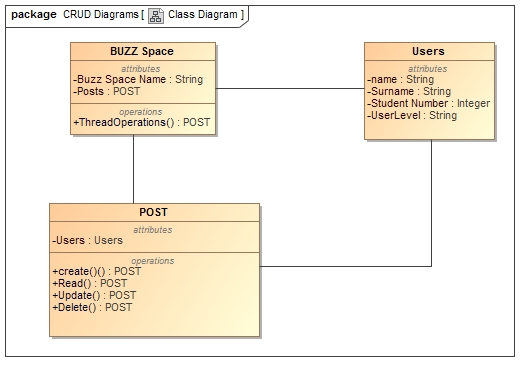
\includegraphics[scale=0.5]{CRUD.jpg}
    	\caption{CRUD Use case diagram}
	\end{figure}
		
\graphicspath{ {../Diagrams/Kyhle/Use_Case_Diagrams/} }	
	\begin{figure}[H]	
    	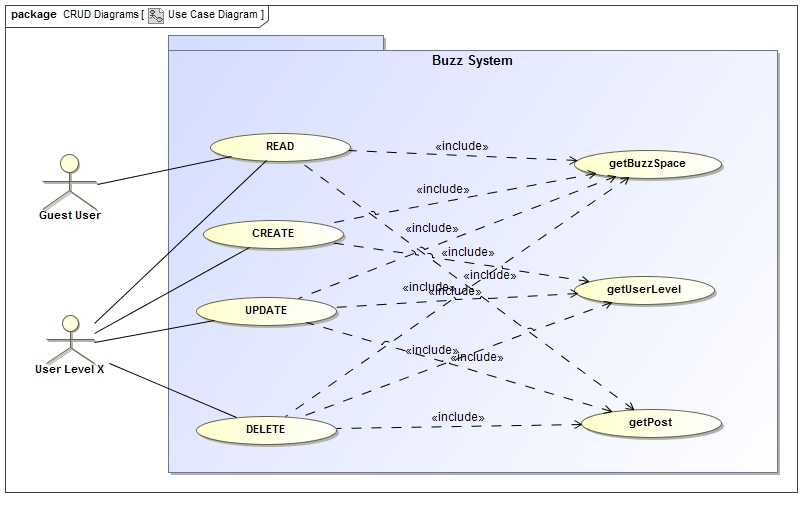
\includegraphics[scale=0.5]{CRUD.jpg}
    	\caption{CRUD Use case diagram}
	\end{figure}
	
\graphicspath{ {../Diagrams/Kyhle/Activity_Diagrams/} }
	\begin{figure}[H]	
    	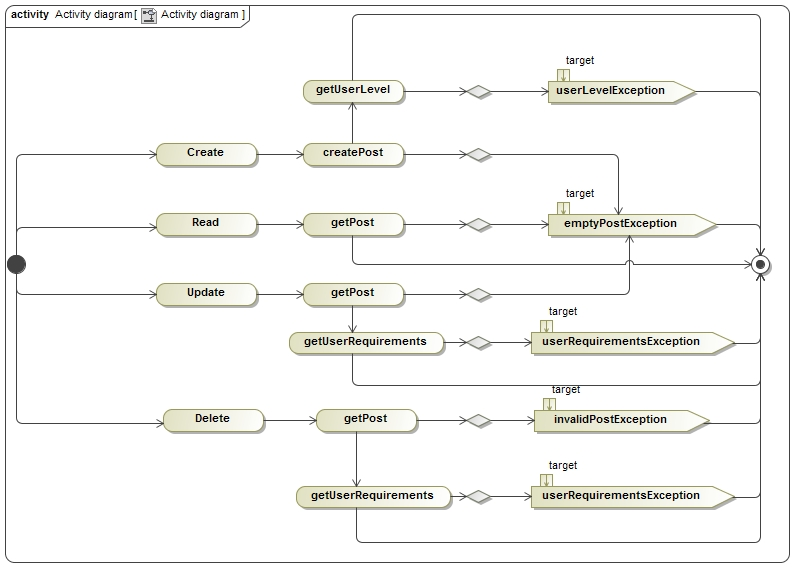
\includegraphics[scale=0.5]{CRUD.jpg}
    	\caption{CRUD Activity diagram}
	\end{figure}

	
\item Tracking read and unread messages:
\begin{itemize}
\item 
\textbf{Purpose:}
The system must keep track of who has read what, and highlight unread messages for each user.
\newline

\item \textbf{Importance:} Critical
\item \textbf{Pre-Conditions: }
	\begin{itemize}
	\item Buzz space must exist.
	\item User must be registered to the buzz system.
	\item User must be logged into the system while viewing the post.
	\end{itemize}

\textbf{Post-Conditions: }
	\begin{itemize}
	\item Post is marked as read.
	\item Post remains unmarked due to some error.
	\end{itemize}

\end{itemize}

\graphicspath{ {../Diagrams/Kyhle/Class_Diagrams/} }	  	
\begin{figure}[H]	
    	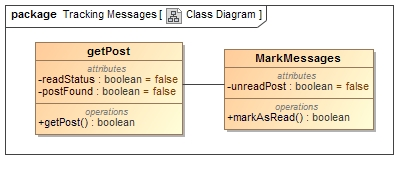
\includegraphics[scale=0.5]{messageTracking.jpg}
    	\caption{Message Tracking Use case diagram}
	\end{figure}

\graphicspath{ {../Diagrams/Kyhle/Use_Case_Diagrams/} }	  	
\begin{figure}[H]	
    	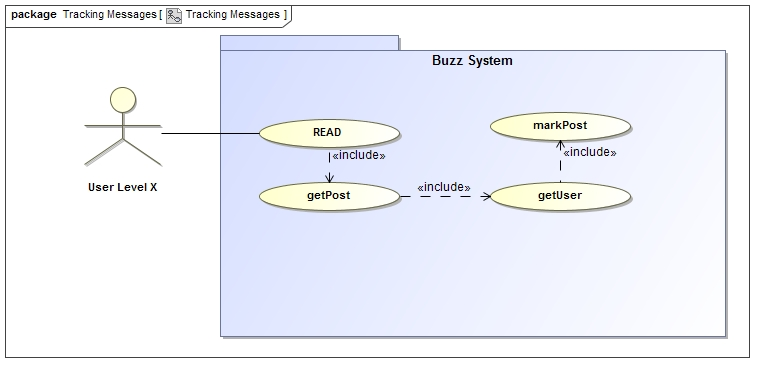
\includegraphics[scale=0.5]{messageTracking.jpg}
    	\caption{Message Tracking Use case diagram}
	\end{figure}
	
\graphicspath{ {../Diagrams/Kyhle/Activity_Diagrams/} }	    	
	\begin{figure}[H]	
    	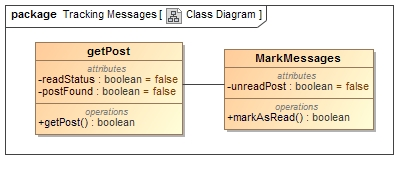
\includegraphics[scale=0.5]{messageTracking.jpg}
    	\caption{Message Tracking Activity diagram}
	\end{figure}
	
\item Message Restrictions: 
\begin{itemize}
\item \textbf{Purpose:}
This deals with the restriction of posting messages.
\newline
\textbf{Limitations:} 
Message length should be restricted. Content type should also be restricted based on level and status of the user posting the message.

\item \textbf{Importance:} Critical\newline
\textbf{Pre-Conditions: }
	\begin{itemize}
	\item Buzz space must exist.
	\item User must be registered to the buzz system.
	\item User must have necessary permissions to create posts of a 		certain length or content type.
	\item Content type and message length must be established by the 		creator of that specific buzz (configurable).
	\end{itemize}

\textbf{Post-Conditions: }
	\begin{itemize}
	\item Post is created.
	\item Post may not have been created due to some error.
	\end{itemize}
\end{itemize}

\graphicspath{ {../Diagrams/Kyhle/Class_Diagrams/} }	    	
	\begin{figure}[H]	
    	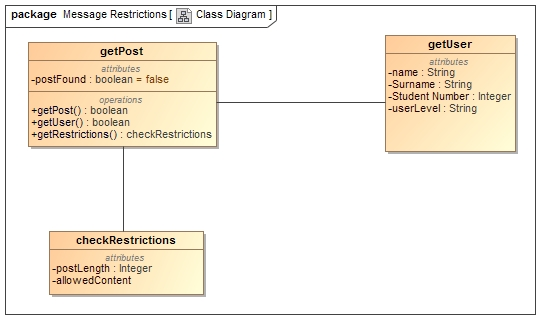
\includegraphics[scale=0.5]{messageRestrictions.jpg}
    	\caption{Message Restrictions Activity diagram}
	\end{figure}
\graphicspath{ {../Diagrams/Kyhle/Use_Case_Diagrams/} }	    	
	\begin{figure}[H]	
    	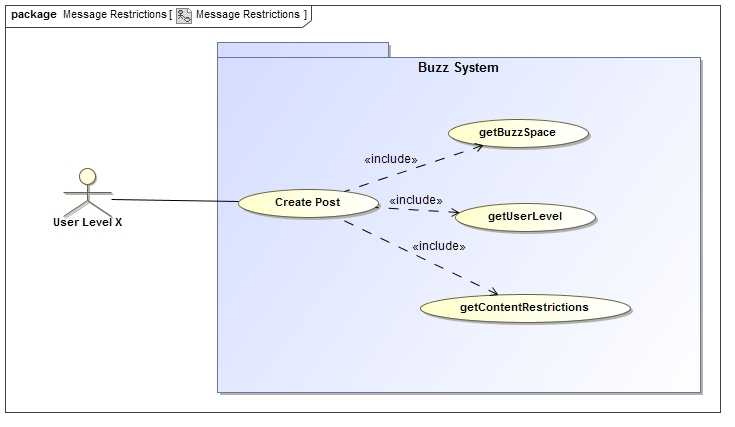
\includegraphics[scale=0.5]{messageRestrictions.jpg}
    	\caption{Message Restrictions Activity diagram}
	\end{figure}
\graphicspath{ {../Diagrams/Kyhle/Activity_Diagrams/} }
	\begin{figure}[H]	
    	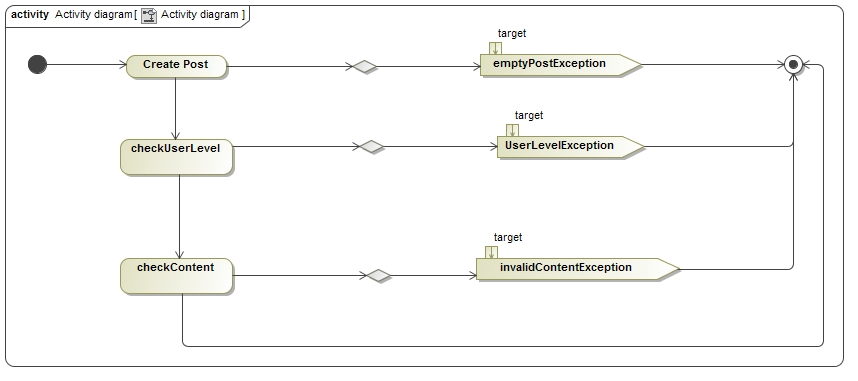
\includegraphics[scale=0.5]{messageRestrictions.jpg}
    	\caption{Message Restrictions Use case diagram}
	\end{figure}
































\item  Restricting users posts depending on user level:
\begin{itemize}	
		\item
		\textbf{Purpose:}
		\newline
		Restrict users to post on specified levels based on their status of the user posting the message.
		\item\textbf{Limitation: }
		\newline
		 There is a limit to number of posts per user on each level.
		 There is a rage of levels from lowest to highest.
		 Staff and the creator have no limitations.
		\item\textbf{Importance:} 
		\newline Important

		\textbf{Pre-Conditions: }
		\newline
		 User must be registered to the buzz system.
	
		\textbf{Post-Conditions: }
		\begin{itemize}
			\item Non-registered user:
			User will not be able to post comment create new threads without acquiring an account.
			\item Low level user:
			When a user is on level x users may only post y number of topic or comments on other users posts per day. New posts can only be posted in pre-		existing threads made by higher level users and no new threads may be made by low level users. 
			\item Medium level user:
			User may add and create any number of posts per day but are limited to the z number of threads that they can create per day.
			\item High level user:
			High level users have no posting restrictions. They made add any number of threads and are not limited to any number of posts per day.
		 	All values are configurable by the Creator.
		 \end{itemize}

	 \graphicspath{ {../Diagrams/Andrew/} }
			 \begin{figure}[H]	
			 	  			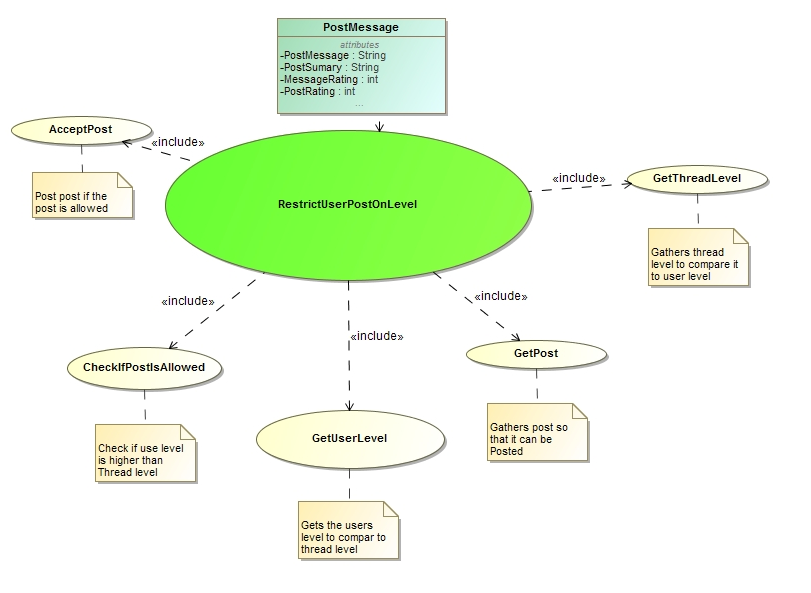
\includegraphics[scale=0.5]{B1UseCase.png}
							\caption{Restricting users posts Use case diagram}
			 	  		\end{figure}

			 	  				 	  			\begin{figure}[H]	
			 	  				 	  				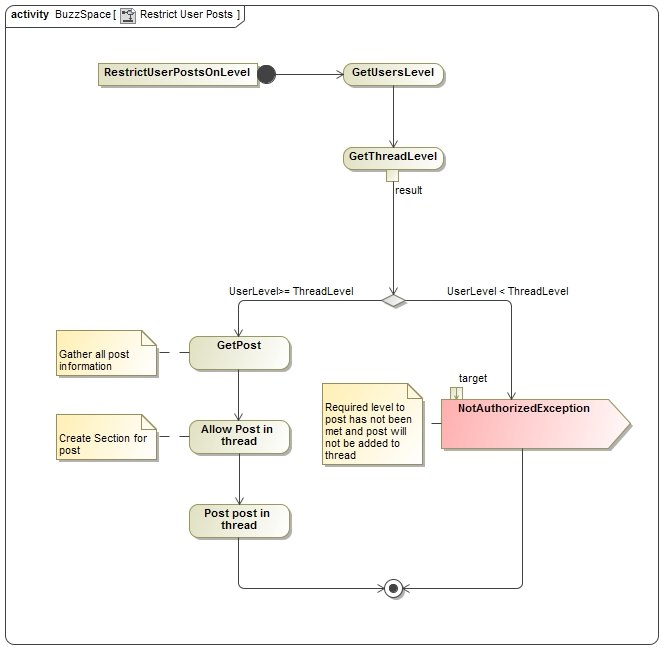
\includegraphics[scale=0.5]{B1Activity.png}
			 	  									\caption{Post restriction Activity diagram}
			 	  				 	  			\end{figure}
			\begin{figure}[H]	
			 	  				 	  						 	  				 	  				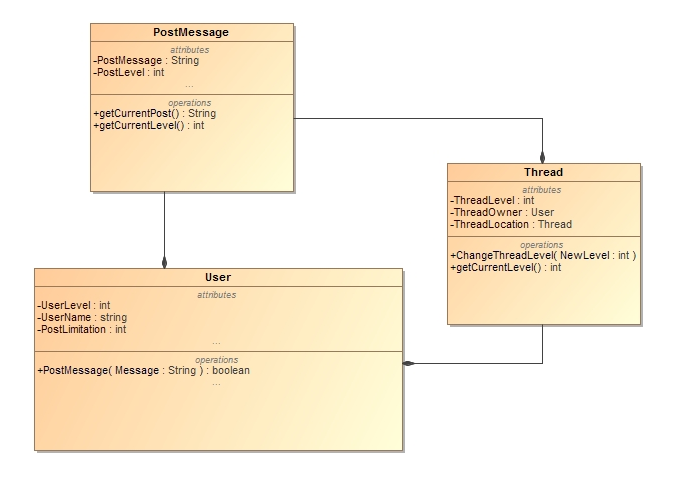
\includegraphics[scale=0.5]{B1ClassDiagram.png}
			 	  				 	  						 	  									\caption{Post restriction Class diagram}
			 	  				 	  						 	  				 	  			\end{figure}
			 	  		
	\newpage	 
		 
\end{itemize}			

 \newpage

\item Staff Being able to edit user posts and a Buzz Space
\begin{itemize}	
	\item 
	\textbf{Purpose:}
	\newline
	Allow staff to manage content i.e. summaries, close or hide threads and move things around.
	\item\textbf{Limitation: }
	\newline
	 Only certain level users can edit other users posts.
	 Cannot edit other peoples posts that are on higher levels.
	\item\textbf{Importance:} 
	\newline
	Important
		

	\textbf{Pre-Conditions: }
	\begin{itemize}
		\item User must be registered to the buzz system.
		\item User must have necessary privileges.
		\item Users may not edit, move or change another user’s \item posts threads or comments that are on the same or on a higher level that they are.
	\end{itemize}
	
	\textbf{Post-Conditions: }
	\begin{itemize}
		\item Staff or high level users:
		User may move threads to their relevant categories. Remove unused or unimportant threads. Lock or close threads so users cannot post within them if the to	pic has been already been answered. Post may be edited to fix error or to remove irrelevant data.
		\item Medium level user:
		User may move posts to the relevant threads but may not edit change or update user’s posts.
		\item Low level and non-registered users:
		User may not edit, move or change another user’s posts threads or comments.
	 	\item All values are configurable by the Creator.
	\end{itemize}

 \graphicspath{ {../Diagrams/Andrew/} }
			 \begin{figure}[H]	
			 	  			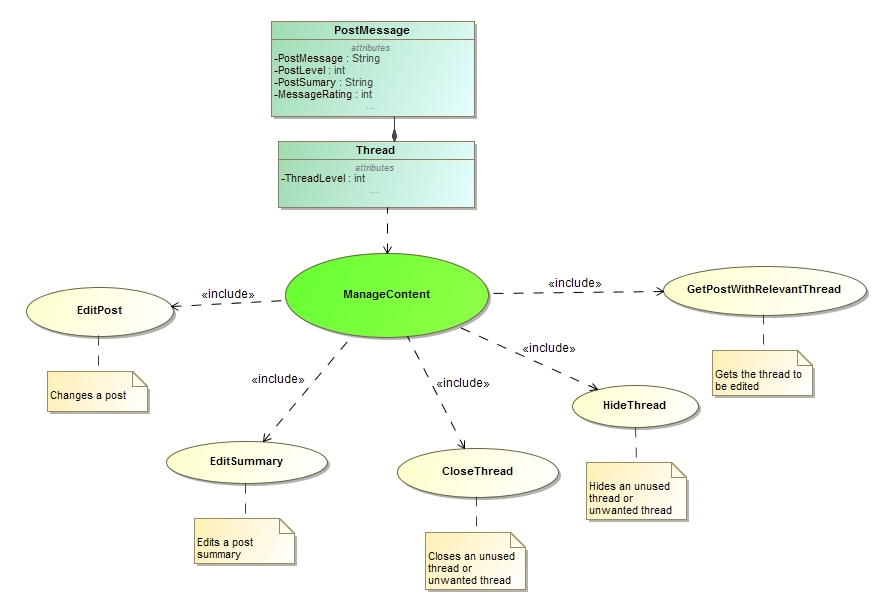
\includegraphics[scale=0.5]{B2UseCase.png}
							\caption{Staff updaing posts Use case diagram}
			 	  		\end{figure}
			 	  					 	  		\begin{figure}[H]		
			 	  					 	  			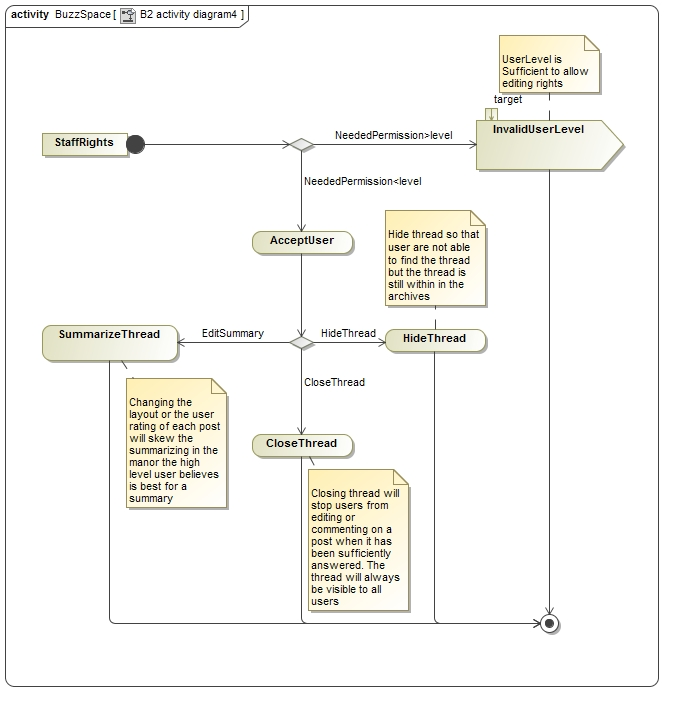
\includegraphics[scale=0.5]{B2Activity.png}
			 	  									\caption{Staff Message updating Activity diagram}
			 	  					 	  		\end{figure}
			 	  					 	  		
			 	  					 	  					 	  					 	  		\begin{figure}[H]		
			 	  					 	  					 	  					 	  			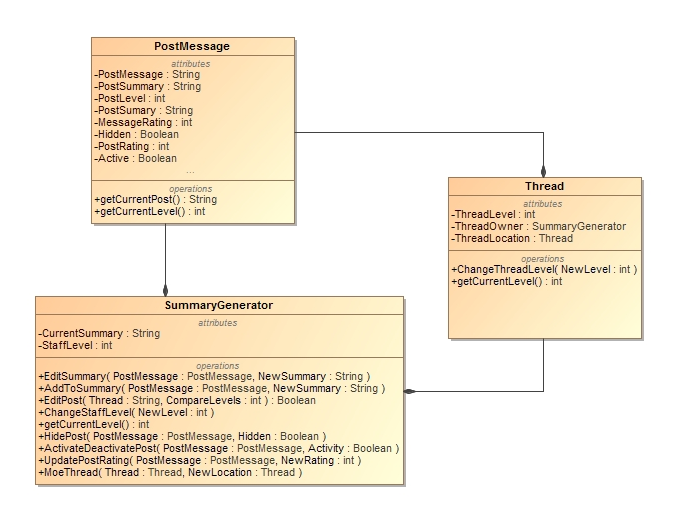
\includegraphics[scale=0.5]{B2ClassDiagram.png}
			 	  					 	  					 	  									\caption{Staff Message updating Class diagram}
			 	  					 	  					 	  					 	  		\end{figure}
			 	  		
	\newpage
			
			 
				
\end{itemize}	
 \newpage
Staff Being able to edit user posts
\item Creating semi-automatic creation of thread summaries.
\begin{itemize}	
	
	
	\item \textbf{Purpose:}
	\newline
	Provide functionality to support semi-automatic creation of thread summaries.
	\item\textbf{Limitation: }
	\newline
	 Threads have to be created.
	Threads have to have a rating.
	Summaries are the reorganization of the thread responses.
	\item\textbf{Importance:} 
	\newline
	Nice-To-Have

	\textbf{Pre-Conditions: }
	\newline Medium, High and Creator may state whether a certain thread may or may not be summarized.
	\newline\textbf{Post-Conditions: }
	\begin{itemize}
		\item When a Thread has been marked for summary then all posts which have been highly rated and important would be moved closer to the top and 	unrelated or unnecessary posts would be move further away from the top to the bottom with all linked comments. 
		\item High level users may override whether the summarized posts are relevant and can manually move the posts to where they best fit.
		\item All levels of users are able to rate posts and comments on how important they see the post.
		\item High level users would get the highest x points per rating.
		\item Medium level users would get the highest y points per rating.
		\item Low level users would get the highest z points per rating.
		\item Non registered users cannot rate posts.
		All values are configurable by the Creator.
	\end{itemize}

 \graphicspath{ {../Diagrams/Andrew/} }
			 \begin{figure}[H]	
			 	  			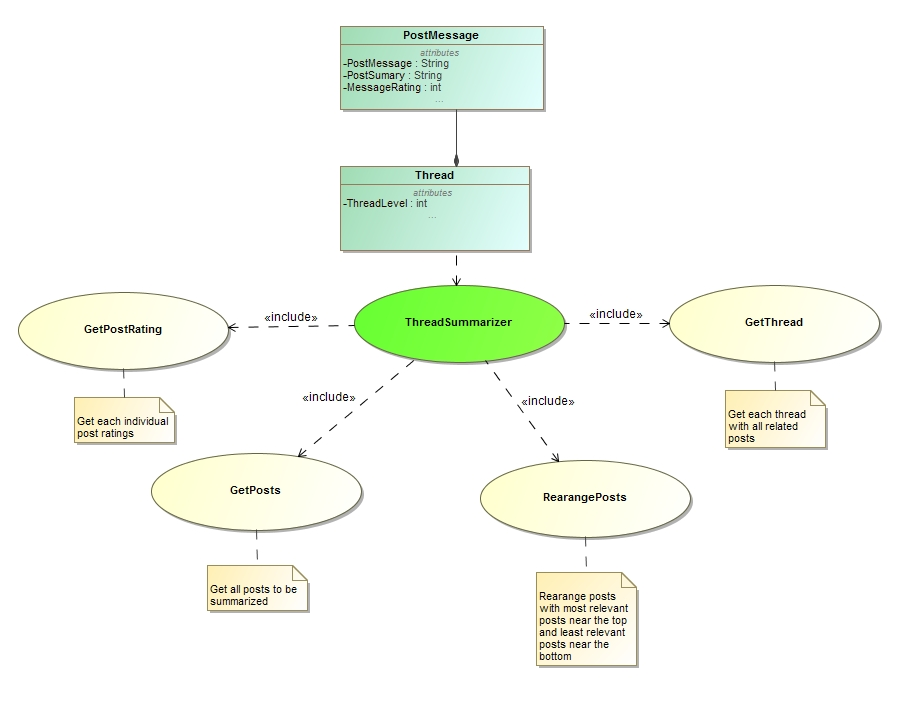
\includegraphics[scale=0.5]{B3UseCase.png}
							\caption{Semi-automatic summaries Use case diagram}
			 	  		\end{figure}
			 	  		
			 	  					 	  		\begin{figure}[H]	
			 	  					 	  			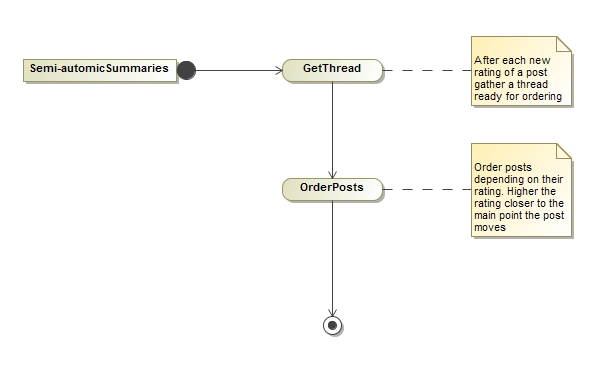
\includegraphics[scale=0.5]{B3Activity.png}
			 	  									\caption{Semi-automatic summaries Activity diagram}
			 	  					 	  		\end{figure}
			 	  					 	  		
			 	  					 	  					 	  		
			 	  					 	  					 	  					 	  		\begin{figure}[H]	
			 	  					 	  					 	  					 	  			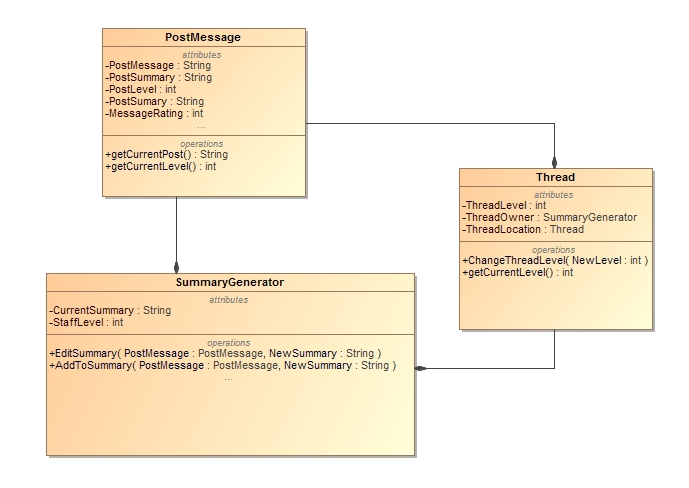
\includegraphics[scale=0.5]{B3ClassDiagram.png}
			 	  					 	  					 	  									\caption{Semi-automatic summaries Class diagram}
			 	  					 	  					 	  					 	  		\end{figure}
	\newpage
			
			 
				
\end{itemize}	

\newpage



				















\item Social Tagging 
\begin{itemize}
\item \textbf{Purpose:}
This deals with social tagging, broad folksnomy type is used
in this social tagging
\newline
\textbf{Limitations:} 
Not all users will be able to tag a buzz
space, Users with higher privileges and lectures will be able to social
tag buzz space

\item \textbf{Importance:} Nice to have\newline
\textbf{Pre-Conditions: }
	\begin{itemize}
	\item Buzz space must exist.
	\item User must be registered to the buzz system.
	\item Buzz space must have a rating from users to be tagged .
	\end{itemize}

\textbf{Post-Conditions: }
	\begin{itemize}
	\item Buzz space tagged with a keyword.
	\item Buzz space available at tag box for fast access.
	\end{itemize}
\end{itemize}

\begin{figure}[H]	
\graphicspath{ {../Diagrams/sfiso/} }
    	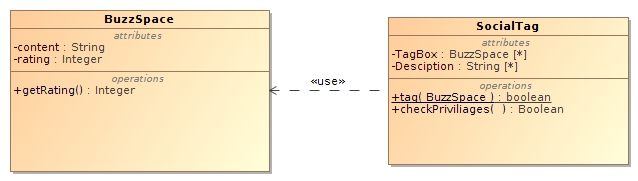
\includegraphics[scale=0.5]{socialC.jpg}
    	\caption{Social Tag class  diagram}
	\end{figure}
	\begin{figure}[H]	
\graphicspath{ {../Diagrams/sfiso/} }
    	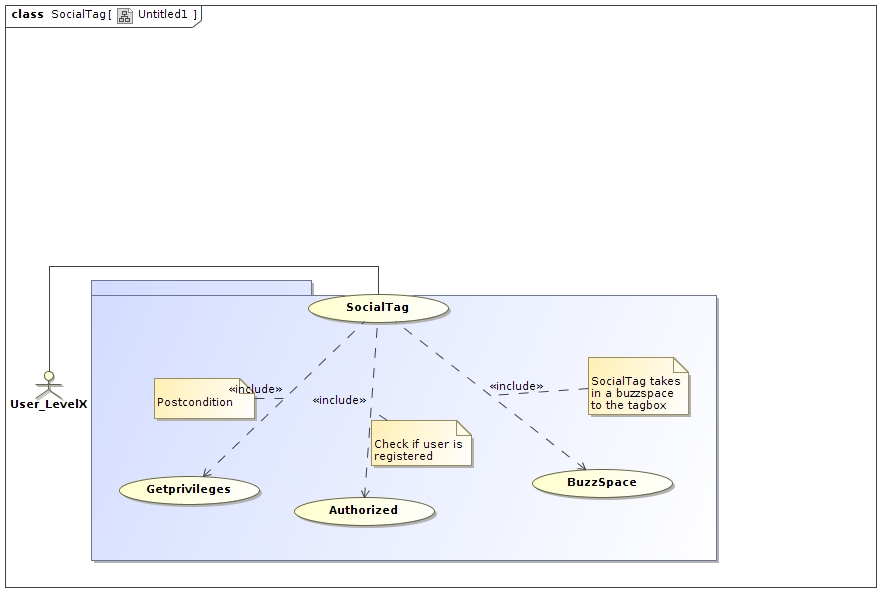
\includegraphics[scale=0.5]{socialtag.jpg}
    	\caption{Social Tag User case diagram}
	\end{figure}

\begin{figure}[H]	
\graphicspath{ {../Diagrams/sfiso/} }
    	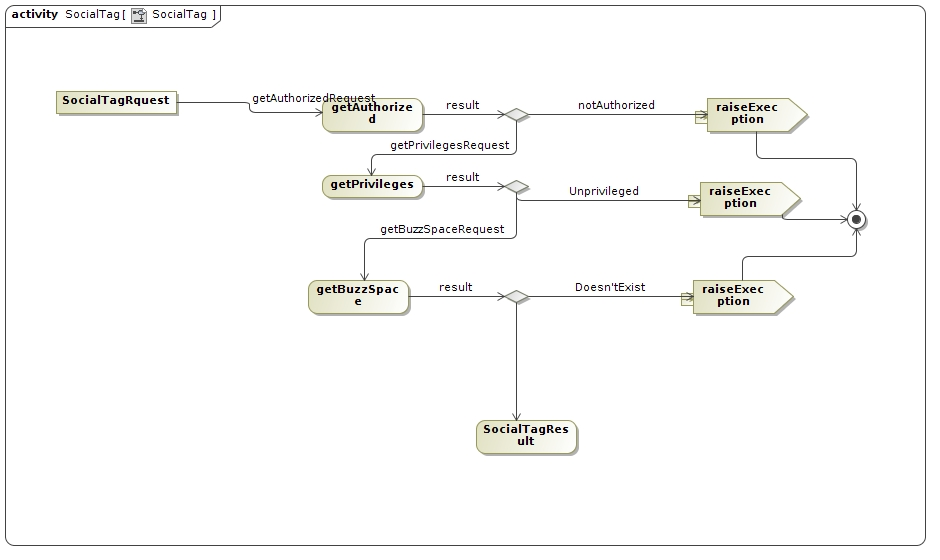
\includegraphics[scale=0.5]{socialA.jpg}
    	\caption{Social Tag Activity  diagram}
	\end{figure}

\item Self organise
\begin{itemize}
\item \textbf{Purpose:}
This deals with self-organization based on social tagging and
allow the user to view according to the base structure, owns structure
or public structure.
\newline
\textbf{Limitations:} 
Users with higher privileges will be able to
organize view to their own structure.

\item \textbf{Importance:}  Nice to have\newline
\textbf{Pre-Conditions: }
	\begin{itemize}
	\item Buzz space must exist.
	\item User must be registered to the buzz system.
	\item Buzz space must have a rating from users to be tagged .
	\item Social tagging must be applied to other buzz space
	\end{itemize}

\textbf{Post-Conditions: }
	\begin{itemize}
	\item Tagged buzz space with higher rating from users will be organized
to be in base structure
	\item Most accessed tagged buzz space will be included in public structure.
	\item Users with buzz space can organize their own structure.
	\end{itemize}
\end{itemize}

\begin{figure}[H]	
\graphicspath{ {../Diagrams/sfiso/} }
    	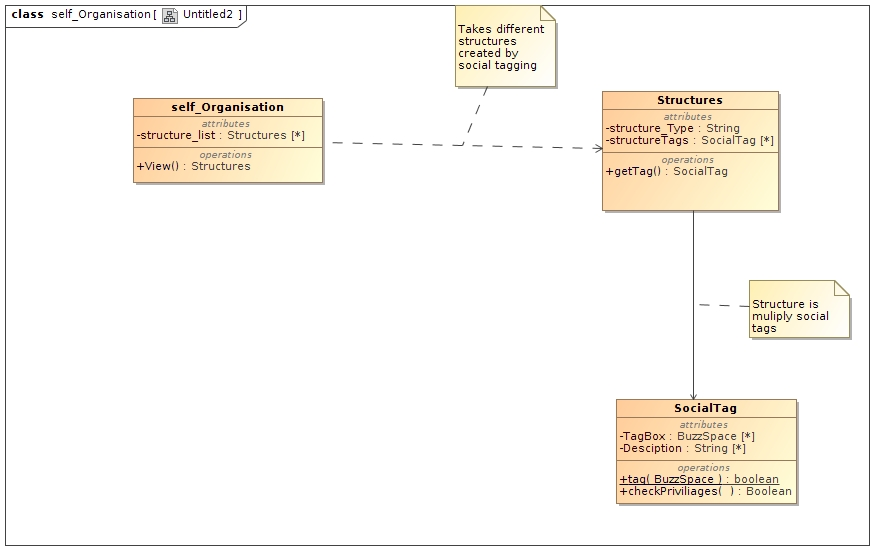
\includegraphics[scale=0.5]{selfC.jpg}
    	\caption{Self organise class diagram}
	\end{figure}

\begin{figure}[H]	
\graphicspath{ {../Diagrams/sfiso/} }
    	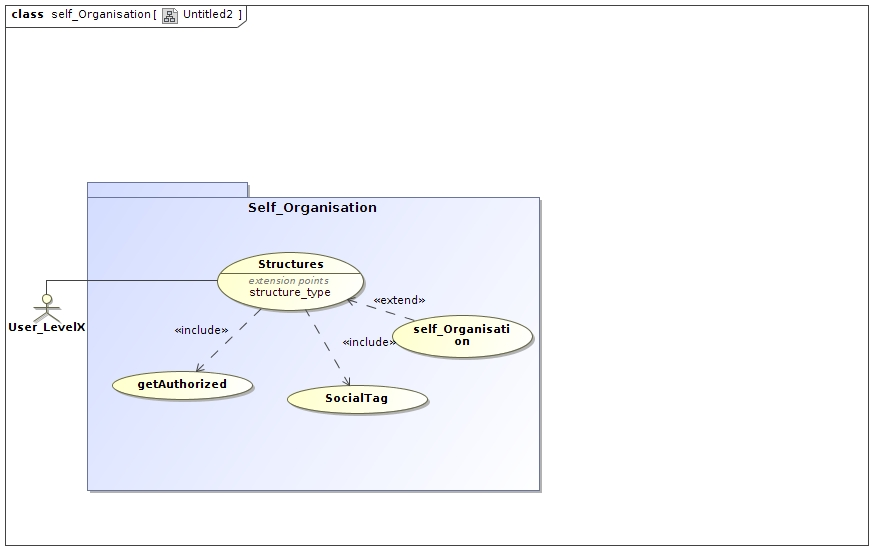
\includegraphics[scale=0.5]{self.jpg}
    	\caption{Self organise User case diagram}
	\end{figure}

\begin{figure}[H]	
\graphicspath{ {../Diagrams/sfiso/} }
    	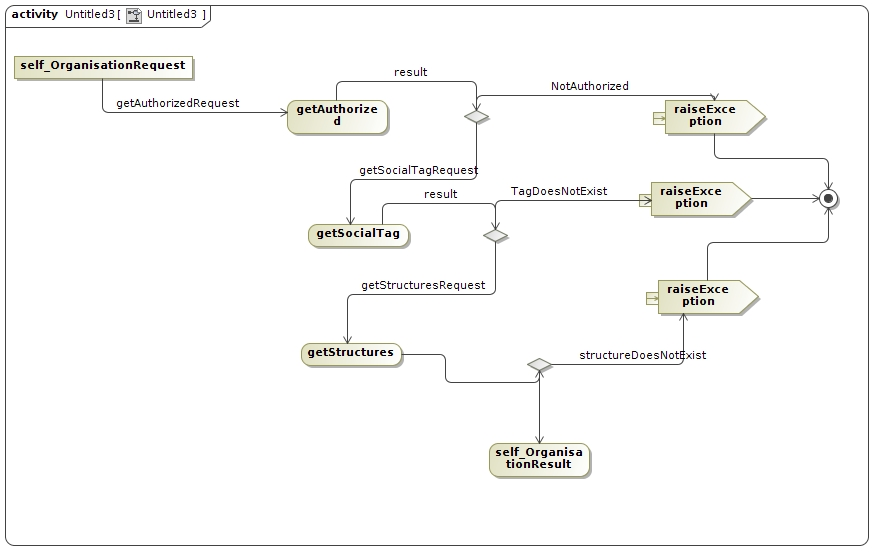
\includegraphics[scale=0.5]{selfA.jpg}
    	\caption{Self organise Activity diagram}
	\end{figure}

\item Buzz Tag
\begin{itemize}
\item \textbf{Purpose:}
This deals with an addition of a read later section, which saves
buzz space with long comments for a user to read later when logged
in and remind the user every time when logged.
\newline
\textbf{Limitations:} 
All users will have this feature by default

\item \textbf{Importance:}  Nice to have\newline
\textbf{Pre-Conditions: }
	\begin{itemize}
	\item Buzz space must exist.
	\item User must be registered to the buzz system.

	\end{itemize}

\textbf{Post-Conditions: }
	\begin{itemize}
	\item Read later section will be created and added on the side of the
users portal
	\item Buzz space reference must be saved in a read later section on the
users portal is the user clicked a buzz space to read later section
	
	\end{itemize}
\end{itemize}
\begin{figure}[H]	
\graphicspath{ {../Diagrams/sfiso/} }
    	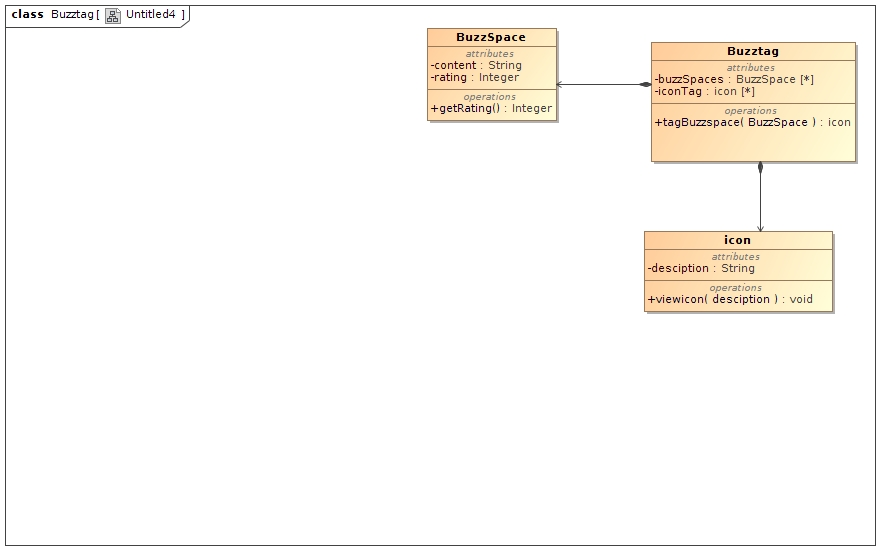
\includegraphics[scale=0.5]{buzzC.jpg}
    	\caption{Buzz Tag class diagram}
	\end{figure}
	
	\begin{figure}[H]	
\graphicspath{ {../Diagrams/sfiso/} }
    	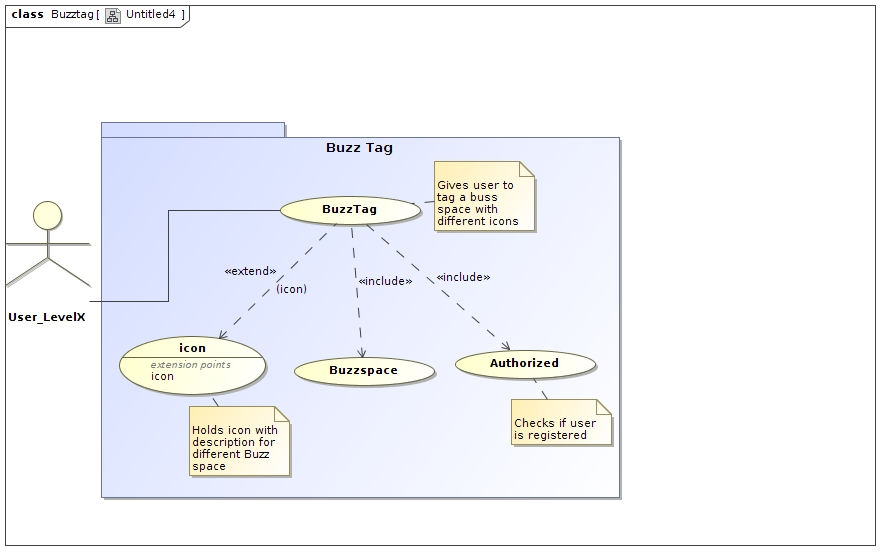
\includegraphics[scale=0.5]{tag.jpg}
    	\caption{Buzz Tag Use case diagram}
	\end{figure}


\begin{figure}[H]	
\graphicspath{ {../Diagrams/sfiso/} }
    	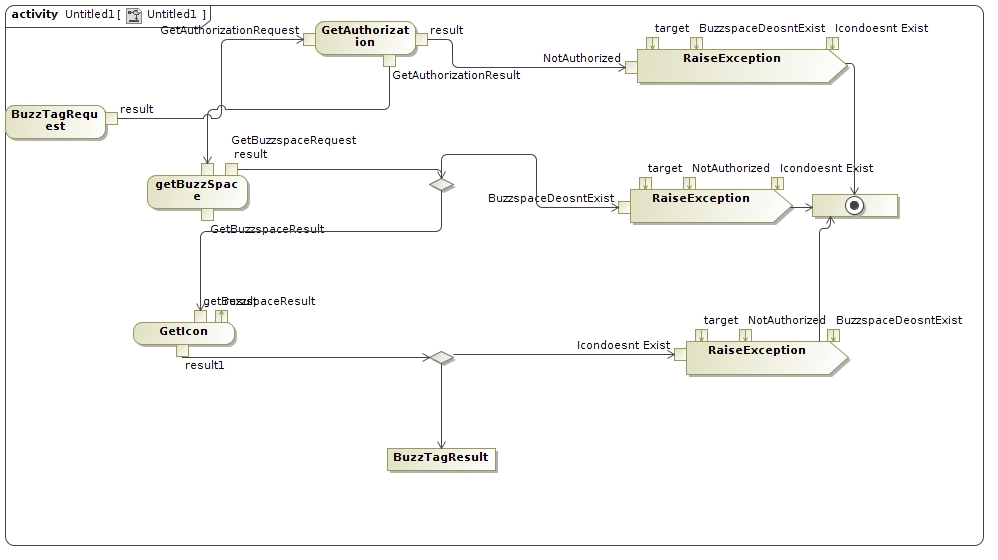
\includegraphics[scale=0.5]{buzzA.jpg}
    	\caption{Buzz Tag Activity diagram}
	\end{figure}

\item Read Later Section
\begin{itemize}
\item \textbf{Purpose:}
This deals with buzz space tagging for least privilege users
,this will help social tagging by providing trending buzz space and
notification system for users who opened buzz space or waiting for a
reply on a comment.
\newline
\textbf{Limitations:} 
All users will have this feature by default

\item \textbf{Importance:} Nice to have\newline
\textbf{Pre-Conditions: }
	\begin{itemize}
	\item Buzz space must exist.
	\item User must be registered to the buzz system.
	\item User optioned for notifications when registering on the buzz system

	\end{itemize}

\textbf{Post-Conditions: }
	\begin{itemize}
	\item Menu will be provided to the user with icons similar to Glyphicons
to describe the buzz space thread for the user to click on.
	\item After user click a certain icon , thread will be rated according to
the icon and each icon have description of the buzz space thread
ranging from lame buzz thread space to must read buzz thread
space and also apply to comments on the buzz space thread .
\item Notification will be send atomically to users read later section to
inform about a new comment on the buzz space user commented
	
	\end{itemize}
\end{itemize}

\begin{figure}[H]	
\graphicspath{ {../Diagrams/sfiso/} }
    	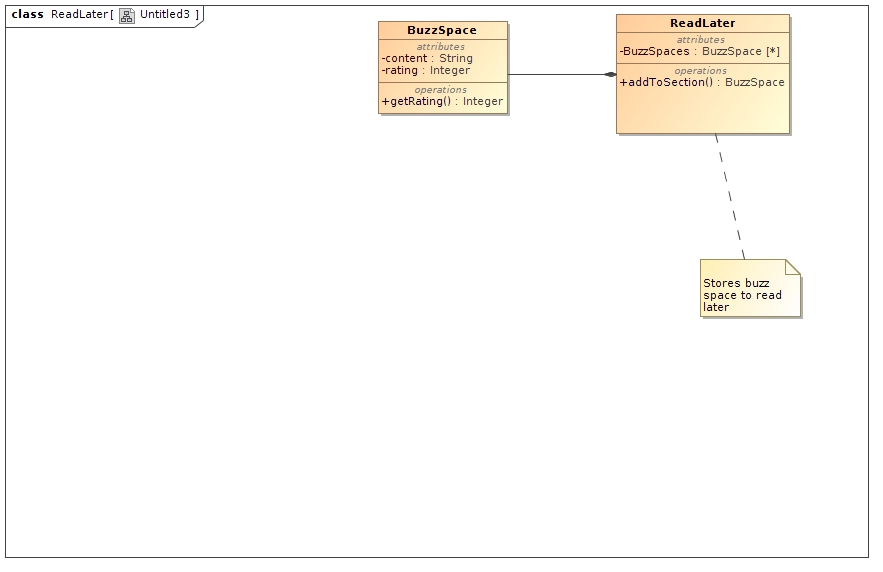
\includegraphics[scale=0.5]{readC.jpg}
    	\caption{Read later section class diagram}
	\end{figure}

\begin{figure}[H]	
\graphicspath{ {../Diagrams/sfiso/} }
    	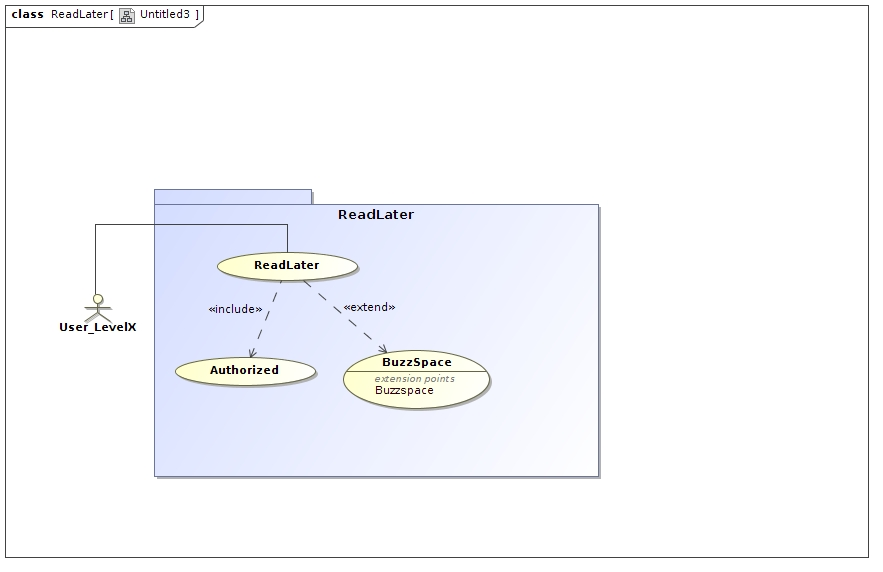
\includegraphics[scale=0.5]{read.jpg}
    	\caption{Read later section Use case diagram}
	\end{figure}
	
	\begin{figure}[H]	
\graphicspath{ {../Diagrams/sfiso/} }
    	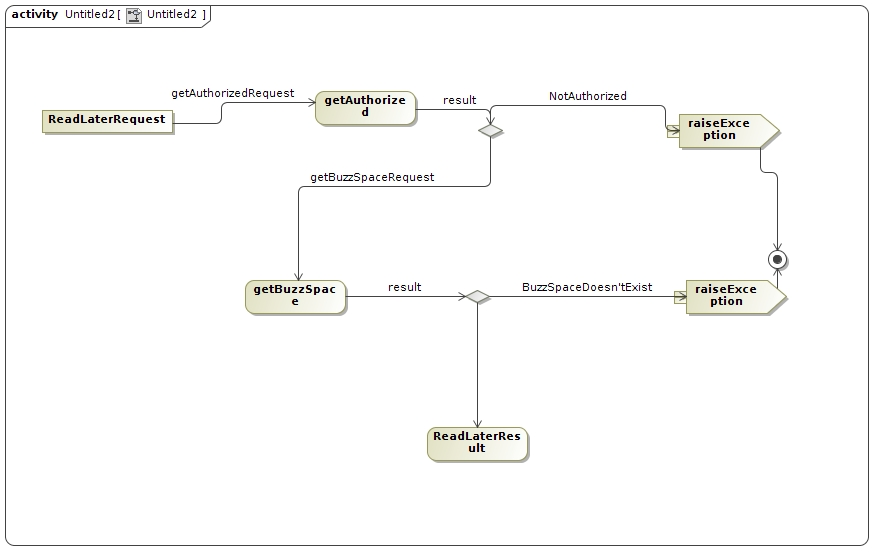
\includegraphics[scale=0.5]{readA.jpg}
    	\caption{Read later section acitivity diagram}
	\end{figure}

\item \textbf{Template messages }
\begin{itemize}
\item \textbf{Purpose: }The management staff must be able to send template messages automatically to individual users or specified groups. These messages would typically be welcoming messages or notification messages. 

	\item  \textbf{Limitation/Exclusions: }
Staff members must be able to add new templates. The staff member should be able to select the receiver(s) based on certain properties.

\item \textbf{Importance:} Nice to have\newline
\textbf{Pre-Conditions: }
	\begin{itemize}
		\item The receiver must be registered to the buzz system.
		\item The sender must be registered as a staff member.
		\item The system must be able to select a certain group based on specific information, to send the group message to.

	\end{itemize}

\textbf{Post-Conditions: }
	\begin{itemize}
		\item The user must be alerted of the message.
		\item The user must not be able to reply to the message.
		\item The user must be able to delete the messages.
		\item The user must not be able to see what other users have received the same message via group messaging.
	\end{itemize}
\end{itemize}

\graphicspath{ {../Diagrams/Maret/usecase/} }	
	\begin{figure}[H]	
    	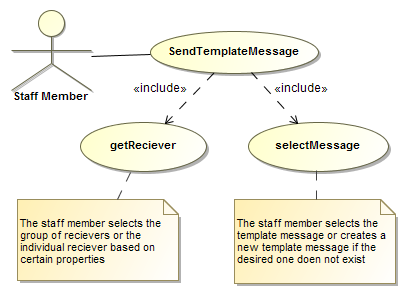
\includegraphics[scale=0.5]{TemplateMessage.png}
    	\caption{Template Message Use Case Diagram}
	\end{figure}
	
\graphicspath{ {../Diagrams/Maret/activity/} }
	\begin{figure}[H]	
    	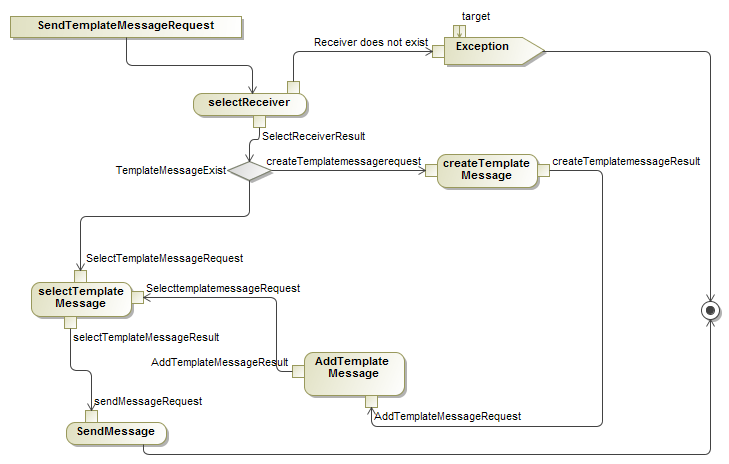
\includegraphics[scale=0.5]{TemplateMessage.png}
    	\caption{Template Message Activity Diagram}
	\end{figure}

\graphicspath{ {../Diagrams/Maret/class/} }
	\begin{figure}[H]	
    	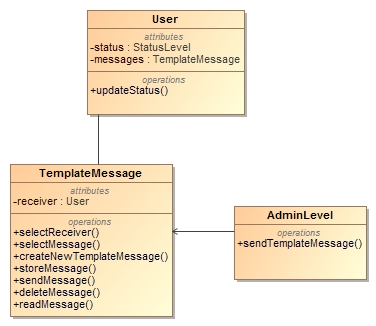
\includegraphics[scale=0.5]{TemplateMessages.jpg}
    	\caption{Template Message Class Diagram}
	\end{figure}		

\item \textbf{Status Updating}
\begin{itemize}
\item \textbf{Purpose: }The system must automatically change the status of a user based on his participation. The system award point to the user based on his actions, these points are then added and influence the users level. The user may lose points for "bad behaviour" and may win points for participation.
 

	\item  \textbf{Limitation/Exclusions: } The status may only change after an action is performed.

\item \textbf{Importance:} Important \newline
\textbf{Pre-Conditions: }
	\begin{itemize}
		\item The user must be registered to the buzz system.
		\item The user must be logged in for his status to be affected by his participation.

	\end{itemize}

\textbf{Post-Conditions: }
	\begin{itemize}
		\item The users points change and as a result of this, his level may change.
		\item The users level, and therefore his privileges, may change when his status change.
		\item The user must be able to view his status.
		\item The users status is public.
	\end{itemize}
\end{itemize}

\graphicspath{ {../Diagrams/Maret/usecase/} }	
	\begin{figure}[H]	
    	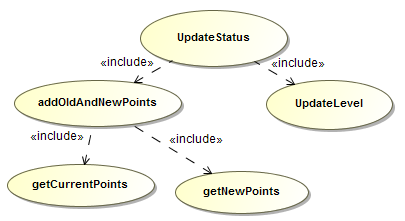
\includegraphics[scale=0.5]{UpdateStatus.png}
    	\caption{Update Status Use Case Diagram}
	\end{figure}
	
\graphicspath{ {../Diagrams/Maret/activity/} }
	\begin{figure}[H]	
    	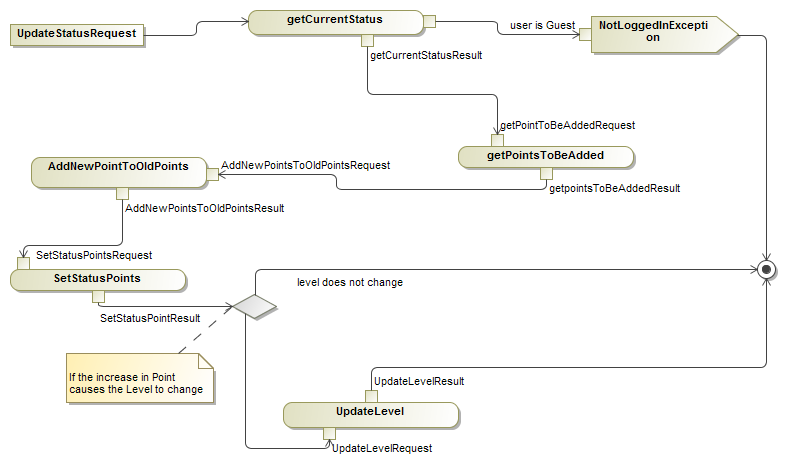
\includegraphics[scale=0.5]{UpdateStatus.png}
    	\caption{Update Status Activity Diagram}
	\end{figure}
	
\graphicspath{ {../Diagrams/Maret/class/} }
	\begin{figure}[H]	
    	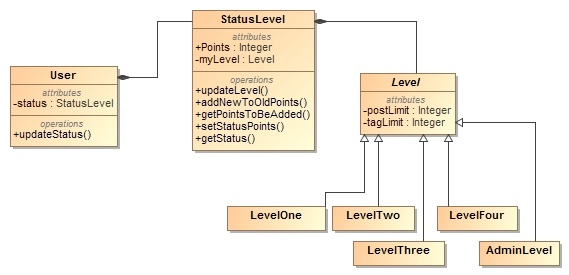
\includegraphics[scale=0.5]{UpdateStatus.jpg}
    	\caption{Update Status Class Diagram}
	\end{figure}

\item \textbf{Integrate with host site}
\begin{itemize}
\item \textbf{Purpose: }The system must be able to integrate with a specified host site.
 
%	\item  \textbf{Limitation/Exclusions: }

\item \textbf{Importance:} Critical \newline
\textbf{Pre-Conditions: }
	\begin{itemize}
		\item The host site must support the technologies of the BuzzSpace system.
		\item TheBuzzSpace system must support the technologies of the host site.

	\end{itemize}

\textbf{Post-Conditions: }
	\begin{itemize}
		\item The system creates the BuzzSpace.
		\item All the data that is on the host site are integrated into the new BuzzSpace.
		\item The users are registered.
		\item The BuzzSpace is stored.
		\item User levels are added.
	\end{itemize}
\end{itemize}

\graphicspath{ {../Diagrams/Maret/usecase/} }	
	\begin{figure}[H]	
    	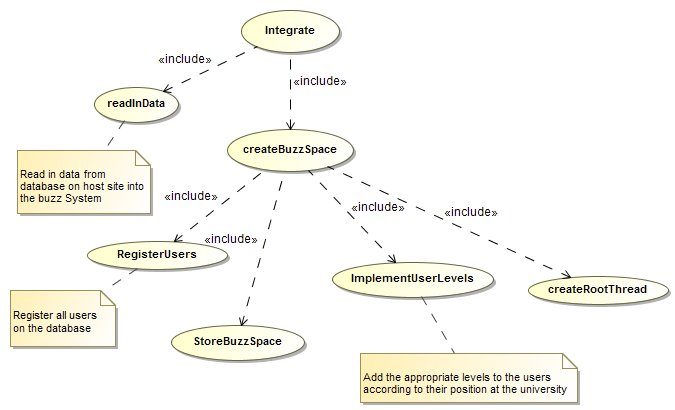
\includegraphics[scale=0.5]{Integrate.png}
    	\caption{Integrate with host site use case diagram}
	\end{figure}
	
\graphicspath{ {../Diagrams/Maret/activity/} }
	\begin{figure}[H]	
    	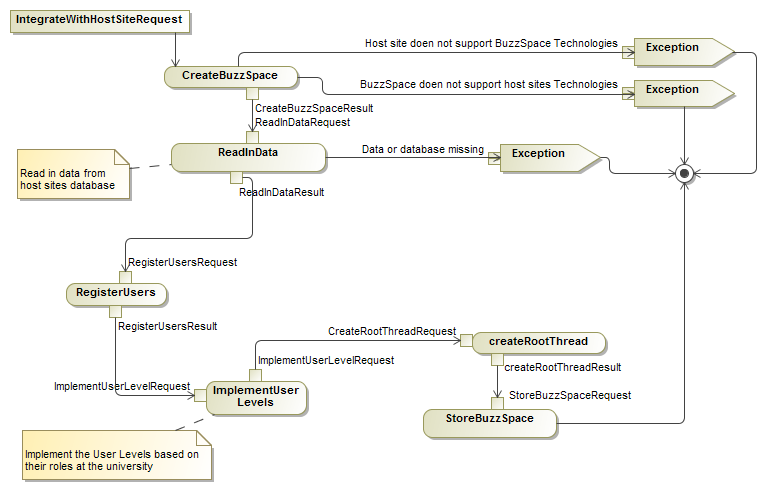
\includegraphics[scale=0.5]{Integrate.png}
    	\caption{Integrate with host site activity diagram}
	\end{figure}
\graphicspath{ {../Diagrams/Maret/class/} }
	\begin{figure}[H]	
    	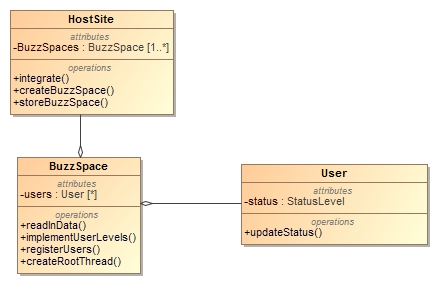
\includegraphics[scale=0.5]{Integrate.jpg}
    	\caption{Integrate with host site class diagram}
	\end{figure}
	
\item \textbf{Search and Filter }
\begin{itemize}
\item \textbf{Purpose: }The website will allow users to search the website for topics and buzz spaces, and then filter those search results by various categories. \newline \newline
	\item  \textbf{Limitation/Exclusions: }
Users will be limited to 4 filter categories, namely: topic, date posted/last updated, buzz space name and rating.
 \graphicspath{ {../Diagrams/Sphe/Search&Filter/} }
 \begin{figure}[H]	
    	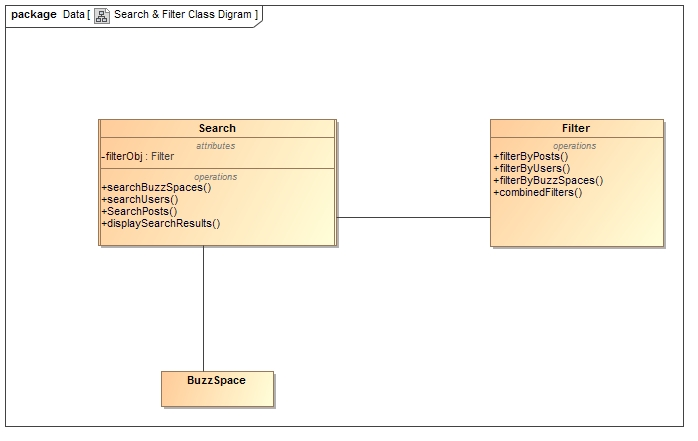
\includegraphics[scale=0.65]{ClassDiagram.jpg}
    	\caption{Search and Filter Class Diagram}
	\end{figure}
\item \textbf{Importance: } Important

\item \textbf{Use case/Service Contracts: } \newline \newline
\end{itemize}
	  \textbf{Post-Conditions: }
	   
	  \begin{itemize}
	  \item Search results are returned
	  \item	Search filters are successfully executed
	  \end{itemize}
	  \graphicspath{ {../Diagrams/Sphe/Search&Filter/} }
	  \begin{figure}[H]	
    	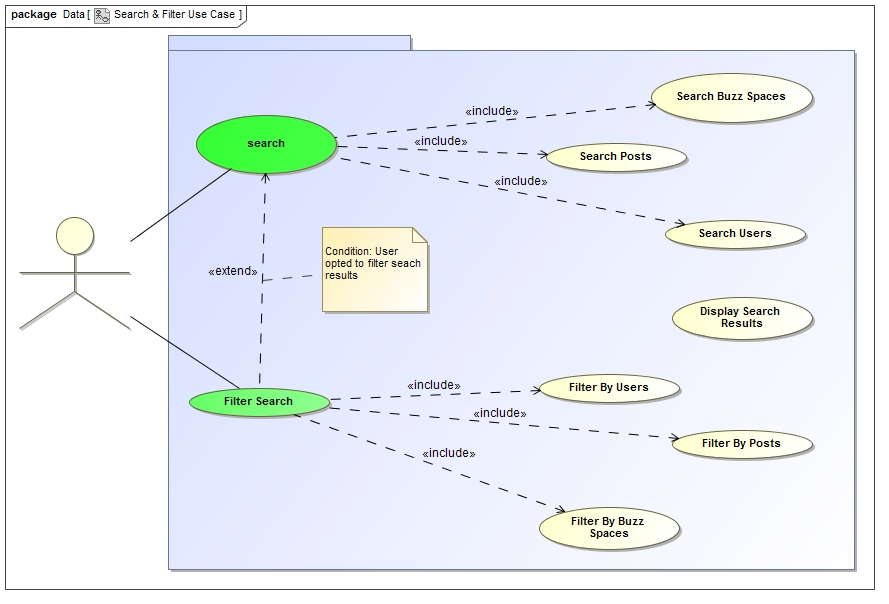
\includegraphics[scale=0.5]{UseCase.jpg}
    	\caption{Search and Filter Use case diagram}
	\end{figure}
	
	\graphicspath{ {../Diagrams/Sphe/Search&Filter/} }
	  \begin{figure}[H]	
    	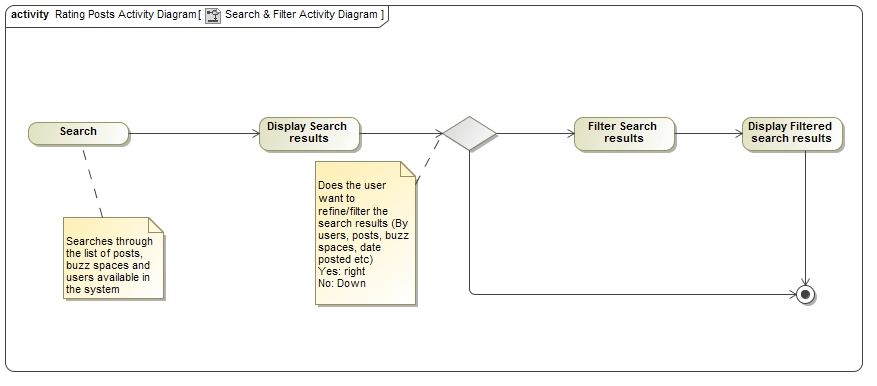
\includegraphics[scale=0.5]{ActivityDiagram.jpg}
    	\caption{Search and Filter Activity Diagram}
	\end{figure}
	
	
	
	 
\item \textbf{Post Rating}
\begin{itemize}
\item \textbf{Purpose: }The website will allow users to evaluate/vote for posts on the website. \newline \newline
	  \textbf{Limitations/Exclusions:} Only users that are logged in to the system and have the privilege rights to evaluate/vote on posts will be allowed to evaluate/vote on posts. Higher Privileged users' votes will push posts higher (or lower) than lower privileged users. \newline \newline
	  \graphicspath{ {../Diagrams/Sphe/PostRatings/} }
	  \begin{figure}[H]	
    	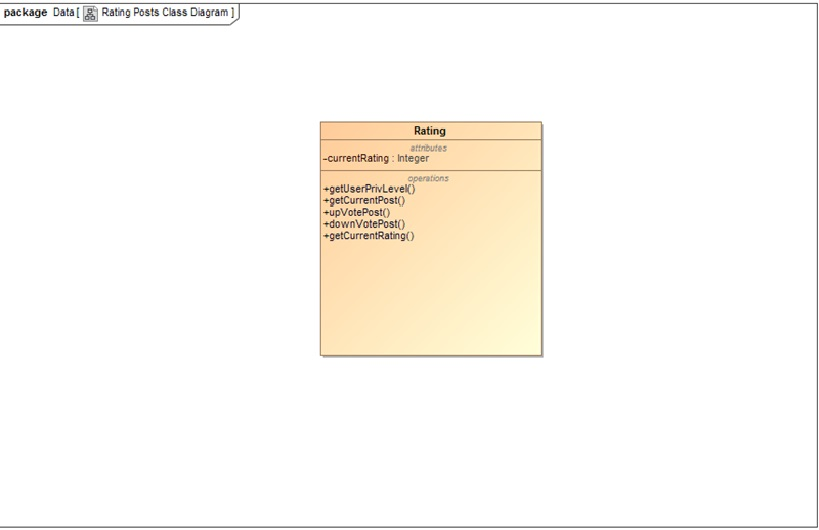
\includegraphics[scale=0.5]{ClassDiagram.jpg}
    	\caption{Post Rating Class Diagram}
	\end{figure}
	  \item \textbf{Importance: } Important \newline \newline
	  \item \textbf{Use Case/Service Contract: } \newline \newline
	  \textbf{Pre-Conditions}
	  \begin{itemize}
	  
	  \item User privilege level allows user to vote for post
	  \item post must exist and not be removed
	  \end{itemize}
	  \textbf{Post Conditions}
	  \begin{itemize}
	  \item Post rating is updated
	  
	  \graphicspath{ {../Diagrams/Sphe/PostRatings/} }
	  \begin{figure}[H]	
    	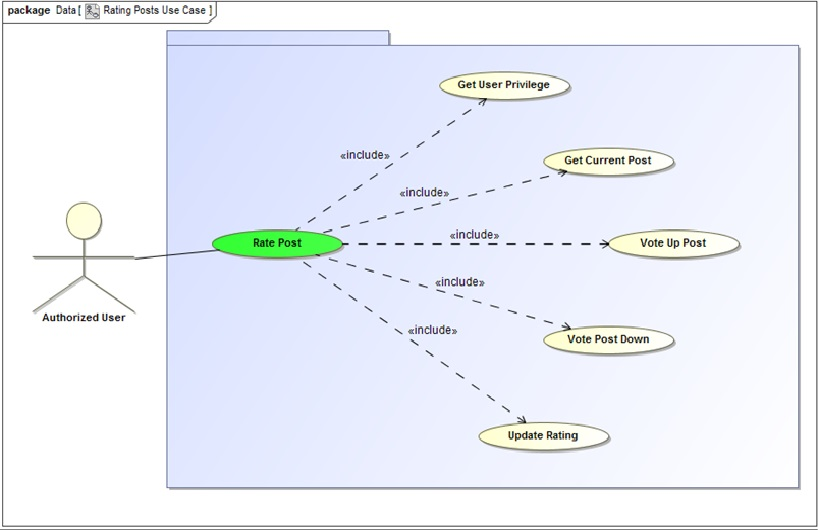
\includegraphics[scale=0.5]{UseCase.jpg}
    	\caption{Post Rating Use case diagram}
    	
    	
	\end{figure}
	\graphicspath{ {../Diagrams/Sphe/PostRatings/} }
	  \begin{figure}[H]	
    	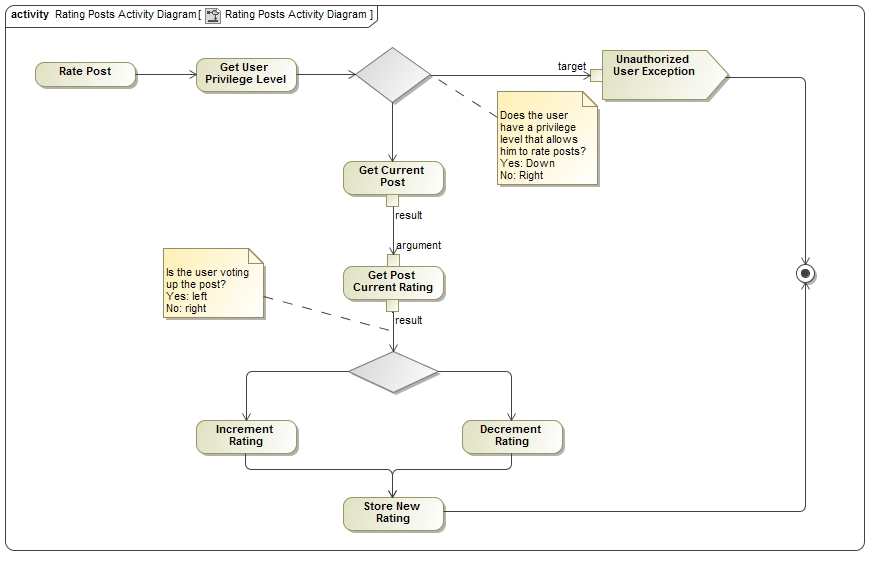
\includegraphics[scale=0.5]{ActivityDiagram.jpg}
    	\caption{Post Rating Activity Diagram}
	\end{figure}
	
	 
	  \end{itemize}
	  \end{itemize}

\newpage

\item \textbf{Statistical Information}

\textbf{Purpose:}
Statistical information created from evaluation to capture average mark of every student within a time frame. Visual reporting of a participants evaluation in correlation to the average of the evaluation of all users or certain groups of users for gamification concept.

\textbf{Limitations/exclusions:} : Not all users may see statistical information of users. Only higher level users may view statistical information and visual reporting of users.

 
\textbf{Importance:} Important.


\textbf{Use case/Service Contracts:} 

\textbf{Pre-Conditions: }
\begin{itemize}
\item User must be connected to buzz.

\item User must be part of discussion or module to be evaluated.

\item User may not be of higher level of the users who monitor the statistical information.


\end{itemize}
 

\textbf{Post-Conditions: }
\begin{itemize}

\item Results and statistical information may not be altered.
\item No more statistical information may be formulated once time period passes.
\item All users may see there statistical information.
\item Statistical information will be represented in a visual representation from that time period.



\end{itemize}

\graphicspath{ {../Diagrams/Matt/Class/} }
	  \begin{figure}[H]	
    	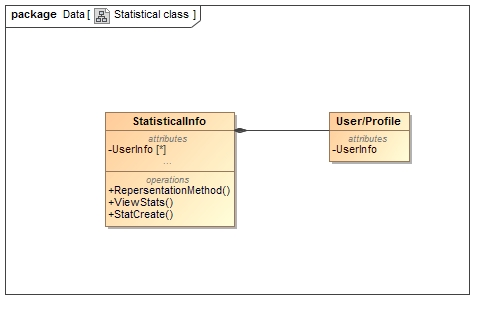
\includegraphics[scale=0.5]{StatisticalClass.jpg}
    	\caption{Statistical information Class Diagram}
	\end{figure}

\graphicspath{ {../Diagrams/Matt/Activity/} }
	  \begin{figure}[H]	
    	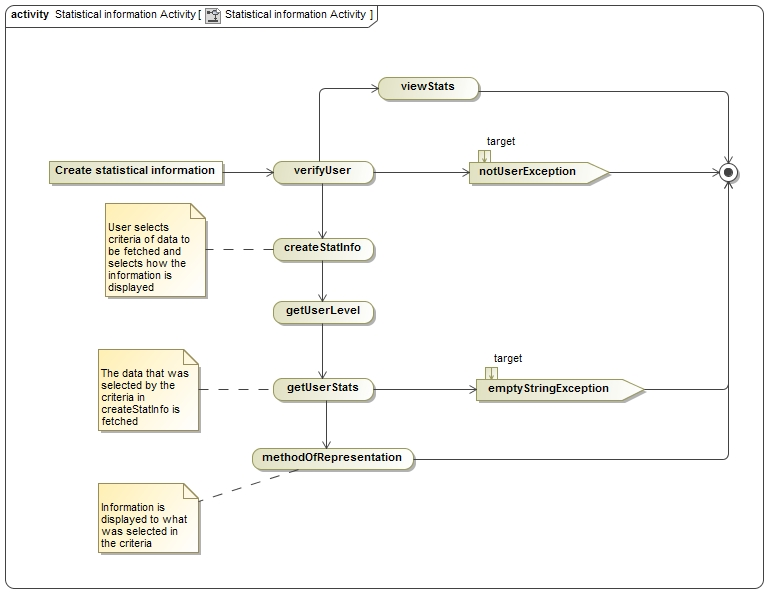
\includegraphics[scale=0.5]{Statisticalinformation.jpg}
    	\caption{Statistical information Activity Diagram}
	\end{figure}

\graphicspath{ {../Diagrams/Matt/Case/} }
	  \begin{figure}[H]	
    	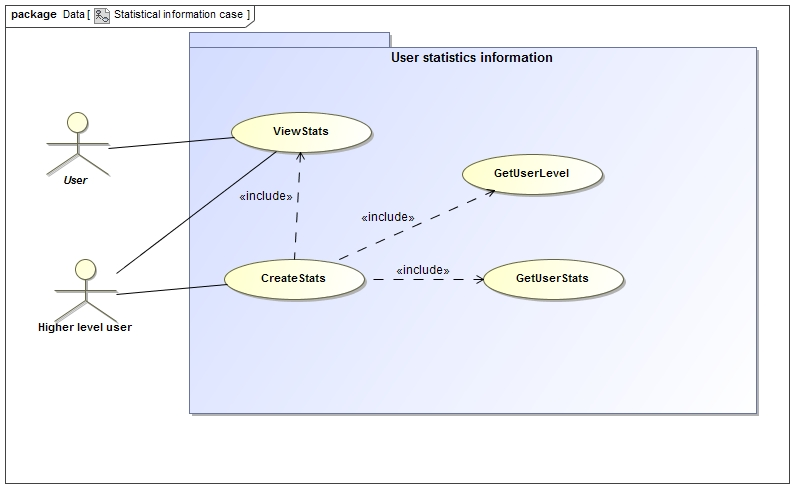
\includegraphics[scale=0.5]{StatisticalinformationCase.jpg}
    	\caption{Statistical information Use case Diagram}
	\end{figure}
	


\item \textbf{Post mark up}

\textbf{Purpose:}
Improved post editor for example text formatting and automatic pretty printing of code in posts.
\newline
\textbf{Limitations/exclusions:} 

Not all users will be able to use these options. Has to be earned. Certain options are available for all users by default.

 
\textbf{Importance:} Nice-To-Have.

 
\textbf{Use case/Service Contracts:} 
\newline
\textbf{Pre-Conditions: }
\begin{itemize}
\item User must be connected to buzz system.
\item User must be of a high enough level.
\item Users must be using the post editor.
\end{itemize}
 

\textbf{Post-Conditions: }
\begin{itemize}

\item Message will be formatted accordingly and marked up (e.g. font colouring,emoticons,various fonts)to how the user wanted. 
\item User must send message to be viewable by other users.
\end{itemize}

\graphicspath{ {../Diagrams/Matt/Class/} }
	  \begin{figure}[H]	
    	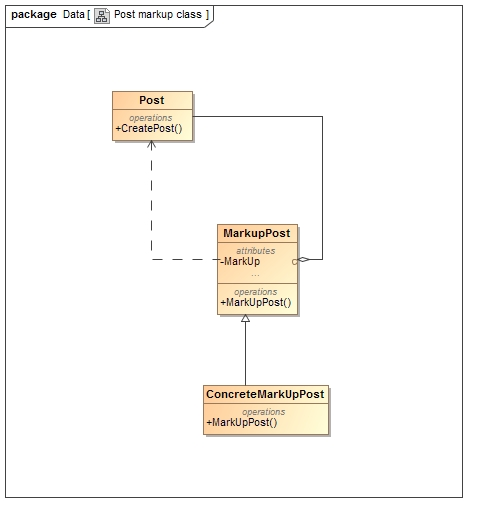
\includegraphics[scale=0.5]{PostmarkupClass.jpg}
    	\caption{Post Markup class Diagram}
	\end{figure}

\graphicspath{ {../Diagrams/Matt/Activity/} }
	  \begin{figure}[H]	
    	\includegraphics[scale=0.5]{PostMarkupActivity.jpg}
    	\caption{Post Markup Activity Diagram}
	\end{figure}
	
\graphicspath{ {../Diagrams/Matt/Case/} }
	  \begin{figure}[H]	
    	\includegraphics[scale=0.5]{Postmarkupcase.jpg}
    	\caption{Statistical information Use case Diagram}
	\end{figure}

\item \textbf{Plagiarism Checker}
\graphicspath{ {../Diagrams/Tienie/Plagiarism/}}
	\begin{itemize}
		\item \textbf{Purpose: }
			This deals with the built in plagiarism checker. It describes the functionality of the plagiarism checker as well as its aims and goals.
		\newline
		\item \textbf{Limitations:} 
		The plagiarism checker is built into the system, and is thus not an optional feature for users posting. However, the checker may be configurable (i.e. turned on and off) by board administrators.
		\item 	\textbf{Importance: } Nice-To-Have
		\item 	\textbf{Pre-Conditions: }
			\begin{itemize}
	  			\item All posts from within the website will need to be available for traversal in text format.
	  			\item A reference collection of documents assumed to be valid will need to be obtained for traversal in text format.
	  			\item A similarity threshold will need to be agreed upon.
		 		\item Access to the Internet (not just Intranet) is a must.
		  		\item A google Search Engine ID and API Key for getting RESTful results to get web search results for comparison in JSON format (Google Custom Search Engine – 100 Free Search Queries Per Day)
		  	\end{itemize}
		\item	\textbf{Post-Conditions}
		  	\begin{itemize}
	  			\item A moderator must be alerted if the plagiarism percentage surpasses the allowed threshold.
		  		\item The percentage of plagiarism detected must be alerted to a moderator if it surpasses the threshold.
	 			\item If plagiarism is detected above the allowed threshold, the post must be highlighted as suspicious.
		  		\item Unique documents scanned must be added to the repository of reference documents.
		  	\end{itemize}
		  	\newpage
	  			\begin{figure}[H]
	  				\caption{Plagiarism Checker Class Diagrams}
    				\includegraphics[scale=0.5]{InputOutput.jpg}
				\end{figure}
				\begin{figure}[H]
					\caption{Plagiarism Checker Use Case Diagram}
		    		\includegraphics[scale=0.4]{UseCase.jpg}
				\end{figure}
				\begin{figure}[H]
					\caption{Plagiarism Checker Activity Diagram}
    				\includegraphics[scale=0.4]{Activity.jpg}
				\end{figure}
	  	\end{itemize}

\graphicspath{ {../Diagrams/Tienie/Netiquette/} }
\newpage
\item Netiquette Checker 
\begin{itemize}
\item \textbf{Purpose: }
This deals with the built in Netiquette checker. It describes the functionality of the Netiquette checker as well as its aims and goals.
\newline
\textbf{Limitations:} 
The netiquette checker is built into the system, and is thus not an optional feature for users posting. However, the checker may be configurable (i.e. turned on and off) by board administrators.
\item 	\textbf{Importance: } Nice-To-Have
	\item	\textbf{Pre-Conditions}
		\begin{itemize}
	  		\item All posts from within the website will need to be available for traversal in text format
	  		\item The netiquette checker will only check the following netiquette rules:
	  		\begin{itemize}
	  			\item Proper Spelling
	  			\item Repetition of Asked Questions
	  			\item Checking all caps
	  			\item Curse word checking
	  			\item Checking for general insults
	  		\end{itemize}
	  		\item We will need a text file containing a large list of commonly used words for the spell checker.
	  		\item We will need a text file containing a large list of commonly used curse words.
			\item We will need a text file containing a large list of words commonly used with the intention of insulting someone.
  		\end{itemize}
  	\item	\textbf{Post-Conditions}
  		\begin{itemize}
	  		\item A moderator must be alerted if a post is detected as violating netiquette.
	  		\item The post must be highlighted to show that it violates netiquette rules.
	  		\item A moderator should be able to hide a post which violates netiquette.
	  		\item The system itself must alert the user of what netiquette rules they have violated as well as give them the opportunity to edit the post and fix them.
	  	\end{itemize}
	  		\begin{figure}[H]
	  			\caption{Netiquette Checker Class Diagram}
	  			\includegraphics[scale=0.35]{NetInputOutput.jpg}
	  		\end{figure}
	  		\begin{figure}[H]
	  			\caption{Netiquette Checker Use Case}
	  			\includegraphics[scale=0.35]{NetUseCase.jpg}
	  		\end{figure}
	  		\begin{figure}[H]
	  			\caption{Netiquette Checker Activity Diagram}
	  			\includegraphics[scale=0.35]{NetProcessDiagram.jpg}
	  		\end{figure}
	  	\end{itemize}

\end{enumerate}

\subsection{Use case Prioritization}
\begin{itemize}
\item \textbf{Critical: }
	\begin{itemize}
		\item CRUD operations.
		\item Tracking read and unread messages.
		\item Message Restrictions.
	\end{itemize}

\item \textbf{Important: }
	\begin{itemize}
		\item Search and Filter.
		\item Post Rating.
		\item Restricting users posts.
		\item Staff Being able to edit user posts.
	\end{itemize}

\item \textbf{Nice-to-Have: }
	\begin{itemize}
		\item Social Tagging.
		\item Self organise.
		\item Buzz Tag.
		\item Read Later Section.
		\item Creating semi-automatic summaries.
		\item Plagiarism Checker
		\item Netiquette Checker
	\end{itemize}
\end{itemize}


\subsection{Process Specifications}
Requirements around the processes which needs to be followed regarding the use cases: \newline

\graphicspath{ {../Diagrams/Kyhle/Activity_Diagrams/} }
	\begin{figure}[H]	
    	\includegraphics[scale=0.5]{CRUD.jpg}
    	\caption{CRUD Activity diagram}
	\end{figure}
    	
	\begin{figure}[H]	
    	\includegraphics[scale=0.5]{messageTracking.jpg}
    	\caption{Message Tracking Activity diagram}
	\end{figure}
	
	\begin{figure}[H]	
    	\includegraphics[scale=0.5]{messageRestrictions.jpg}
    	\caption{Message Restrictions Activity diagram}
	\end{figure}

					
	
	\graphicspath{ {../Diagrams/Sphe/Search&Filter/} }
	  \begin{figure}[H]	
    	\includegraphics[scale=0.65]{ActivityDiagram.jpg}
    	\caption{Search and Filter Activity Diagram}
	\end{figure}
	
	\graphicspath{ {../Diagrams/Sphe/PostRatings/} }
	  \begin{figure}[H]	
    	\includegraphics[scale=0.65]{ActivityDiagram.jpg}
    	\caption{Post Rating Use Activity Diagram}
	\end{figure}
	
	\begin{figure}[H]	
\graphicspath{ {../Diagrams/sfiso/} }
    	\includegraphics[scale=0.5]{socialA.jpg}
    	\caption{Social Tag  Activity Diagram}
	\end{figure}
	\begin{figure}[H]	
\graphicspath{ {../Diagrams/sfiso/} }
    	\includegraphics[scale=0.5]{buzzA.jpg}
    	\caption{Buzz Tag  Activity Diagram}
	\end{figure}

	\begin{figure}[H]	
\graphicspath{ {../Diagrams/sfiso/} }
    	\includegraphics[scale=0.5]{selfA.jpg}
    	\caption{Self organise Activity Diagram}
	\end{figure}

	\begin{figure}[H]	
\graphicspath{ {../Diagrams/sfiso/} }
    	\includegraphics[scale=0.5]{readA.jpg}
    	\caption{Read later section Activity Diagram}
	\end{figure}




\subsection{Domain Model}
\graphicspath{ {../Diagrams/} }
	  \begin{figure}[H]	
    	\includegraphics[scale=0.32]{Domain.jpg}
    	\caption{Complete System Domain Model}
	\end{figure}

\end{document}
